\documentclass[a4paper, amsfonts, amssymb, amsmath, reprint, showkeys, nofootinbib, twoside]{revtex4-1}
\usepackage[english]{babel}
\usepackage[utf8]{inputenc}
\usepackage[colorinlistoftodos, color=green!40, prependcaption]{todonotes}
\usepackage[pdftex, pdftitle={Article}, pdfauthor={Author}]{hyperref}
\usepackage{amsthm}
\usepackage{mathtools}
\usepackage{physics}
\usepackage{xcolor}
\usepackage{caption}
\usepackage{hyperref}
%\hypersetup{colorlinks=true, linkcolor=blue, urlcolor = blue}
\usepackage{amsmath}
\usepackage{amssymb}
\usepackage{graphicx}
\graphicspath{Images}
\usepackage[left=23mm,right=13mm,top=35mm,columnsep=15pt]{geometry} 
\usepackage{adjustbox}
\usepackage{placeins}
\usepackage[T1]{fontenc}
\usepackage{float}
%\usepackage{longtable}
\usepackage{csquotes}
\usepackage{refstyle}
\usepackage{lipsum}
\usepackage{booktabs}



\begin{document}

\title{Splitting of Sodium D lines using diffraction grating}
\author{Swaroop Ramakant Avarsekar}
\email{swaroop.avarsekar@niser.ac.in}
\affiliation{School of Physical Sciences, National Institute of Science Education and Research, HBNI, Jatni -752050, India}
\date{\today}
	
\maketitle

\section{Introduction and Theory}
Fraunhofer observed the absorption spectral lines of the sun and labeled those lines with letters from A-K. A doublet line at 589 nm and 589.6 nm identified as D lines in the sodium emission spectrum was observed. 
\begin{figure}[H] %  figure placement: here, top, bottom, or page
	\centering
	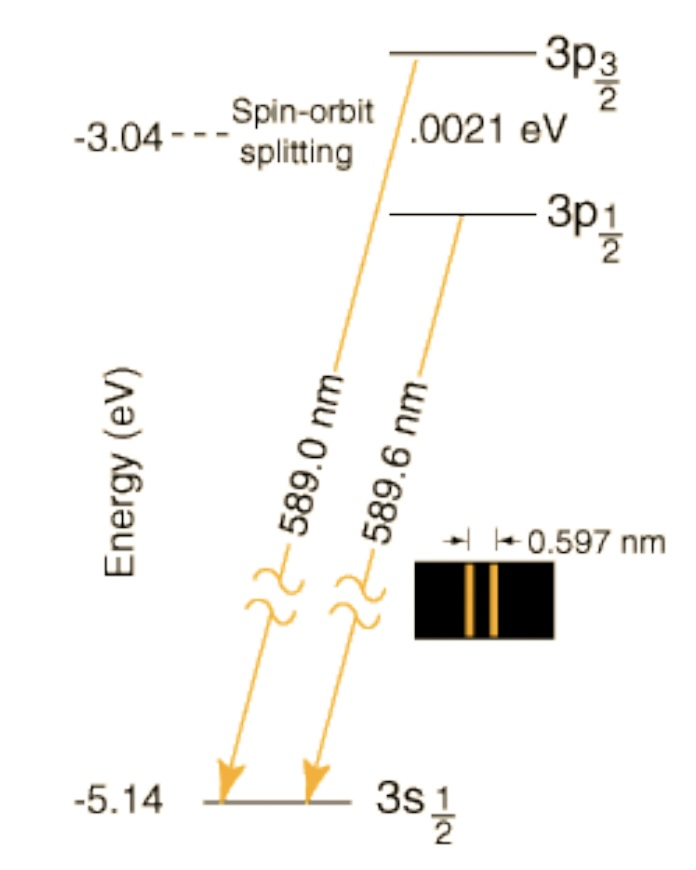
\includegraphics[width=8cm, height=8cm]{1} 
	\caption{Sodium Doublet due to spin orbit coupling}
	\label{1}
\end{figure}

The doublet arises due to transition from 3p to 3s levels. The 3p levels are split into states with angular momentum j=3/2 and j=1/2 due to spin orbit effect, by the magnetic energy of the electron spin in presence of internal magnetic field due to orbital motion.

Using diffraction grating wavelength of the sodium D lines can be calculated with the help of spectrometer. Diffraction grating is the arrangement of the numerous parallel slits (N) with equal width (e) and spacing (b). The grating element is defined as (e+b) and N is the number of slits per unit length (N=1/(e+b)). Angular dispersive power of diffraction grating is defined as rate of change of angle of  diffraction with change in wavelength. The principal maxima is given by 
\begin{equation}
	(e+b)sin \theta=\pm m \lambda
\end{equation}

where $m$ is the order of principal maximum and $\theta$ is the angle of diffraction.

The angular dispersive power is given by 
\begin{equation}
	\frac{d\theta}{d\lambda}=\frac{m}{(e+b)cos\theta}
\end{equation}
\section{Experiment}
\subsection{Apparatus}
For this experiment we need spectrometer, diffraction grating and sodium lamp source with power source. Prism is used to setup the spectrometer.

\begin{figure}[H] %  figure placement: here, top, bottom, or page
	\centering
	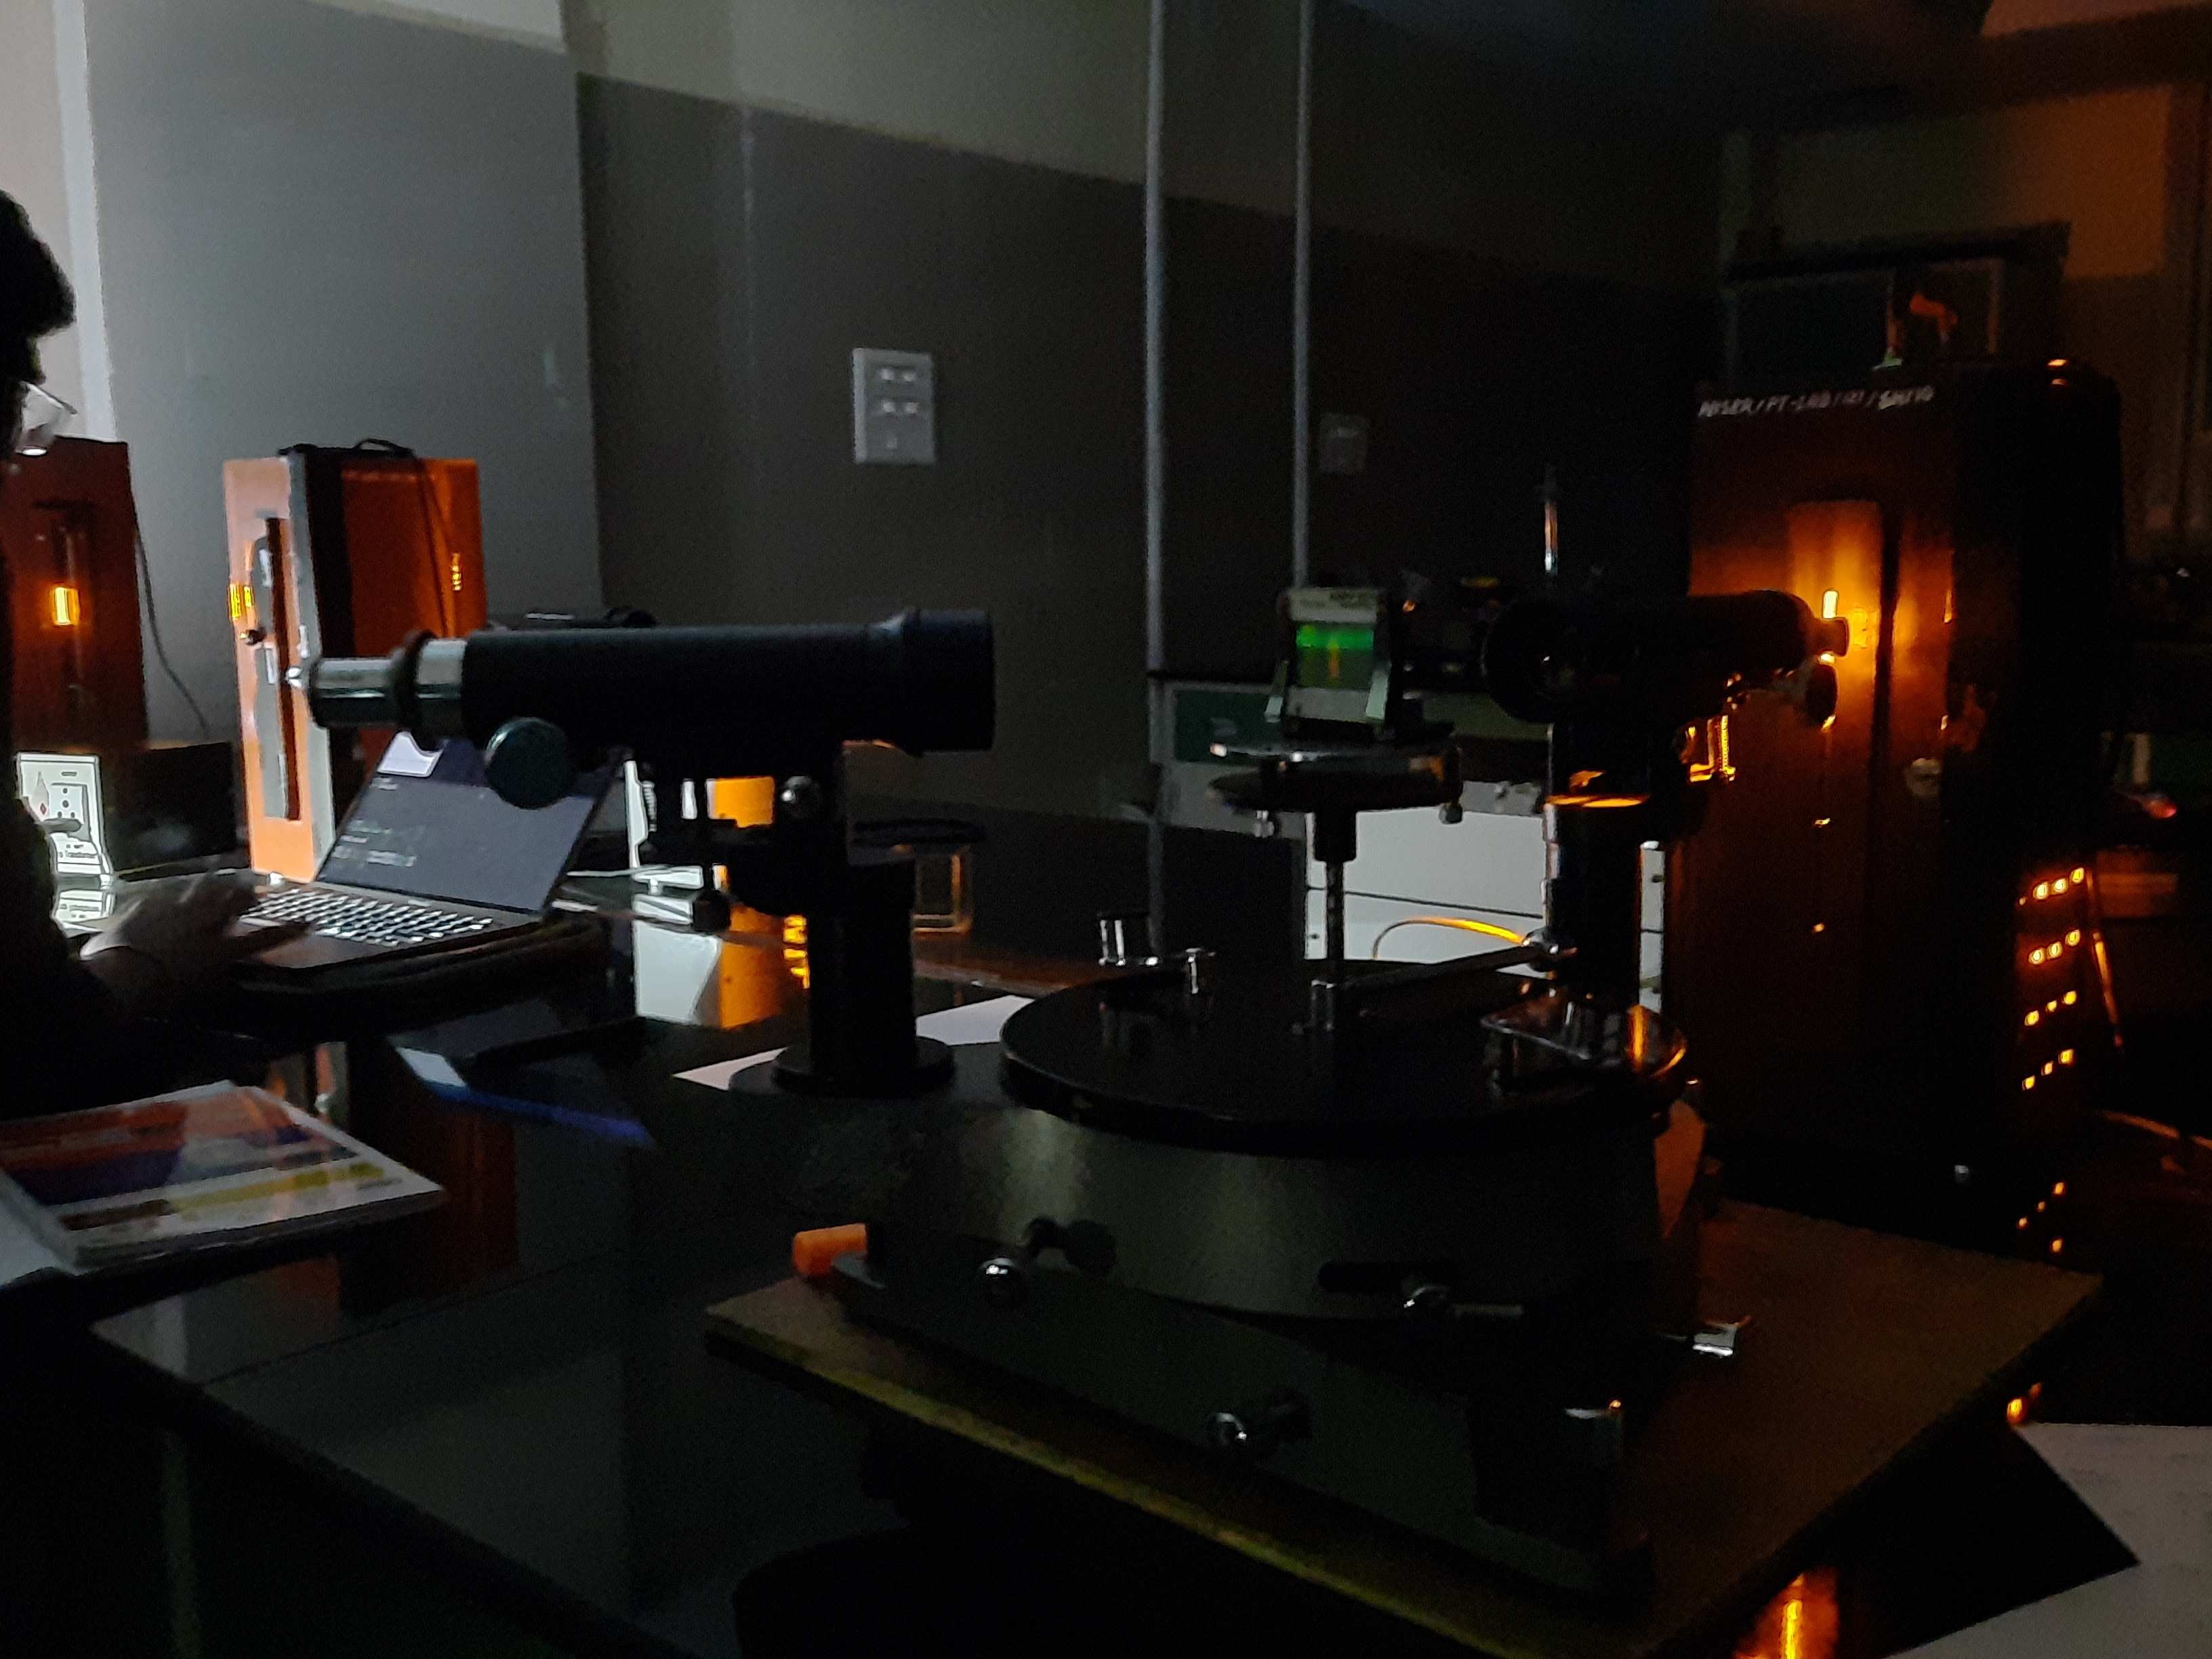
\includegraphics[width=8cm, height=8cm]{2} 
	\caption{Experimental Setup in Laboratory}
	\label{1}
\end{figure}
\subsection{Procedure}

Focus the parallel rays from slit by Schuster's method. Fix the grating on the prism table and observe the slit through telescope aligned along the collimator. The first order and second order diffraction maxima are visible in at the angles left and right side of the collimator. The reading of vernier is taken for the sodium doublet from the edge of the line and moving in the same direction.  Determine the diffraction angle and hence wavelength of the sodium doublet.
\subsection{Precautions}
\begin{enumerate}
\item{Make sure you lock the spectrometer while measuring taking the readings.}
\item{Keep the apparatus free from mechanical disturbances.}
\item{Move the spectrometer in one direction to avoid backlash error.}
\item{Once the collimator and telescope is adjusted for parallel rays, focusing should not be disturbed.}
\end{enumerate}

\subsection{Observations and Analysis}

\begin{figure}[H] %  figure placement: here, top, bottom, or page
	\centering
	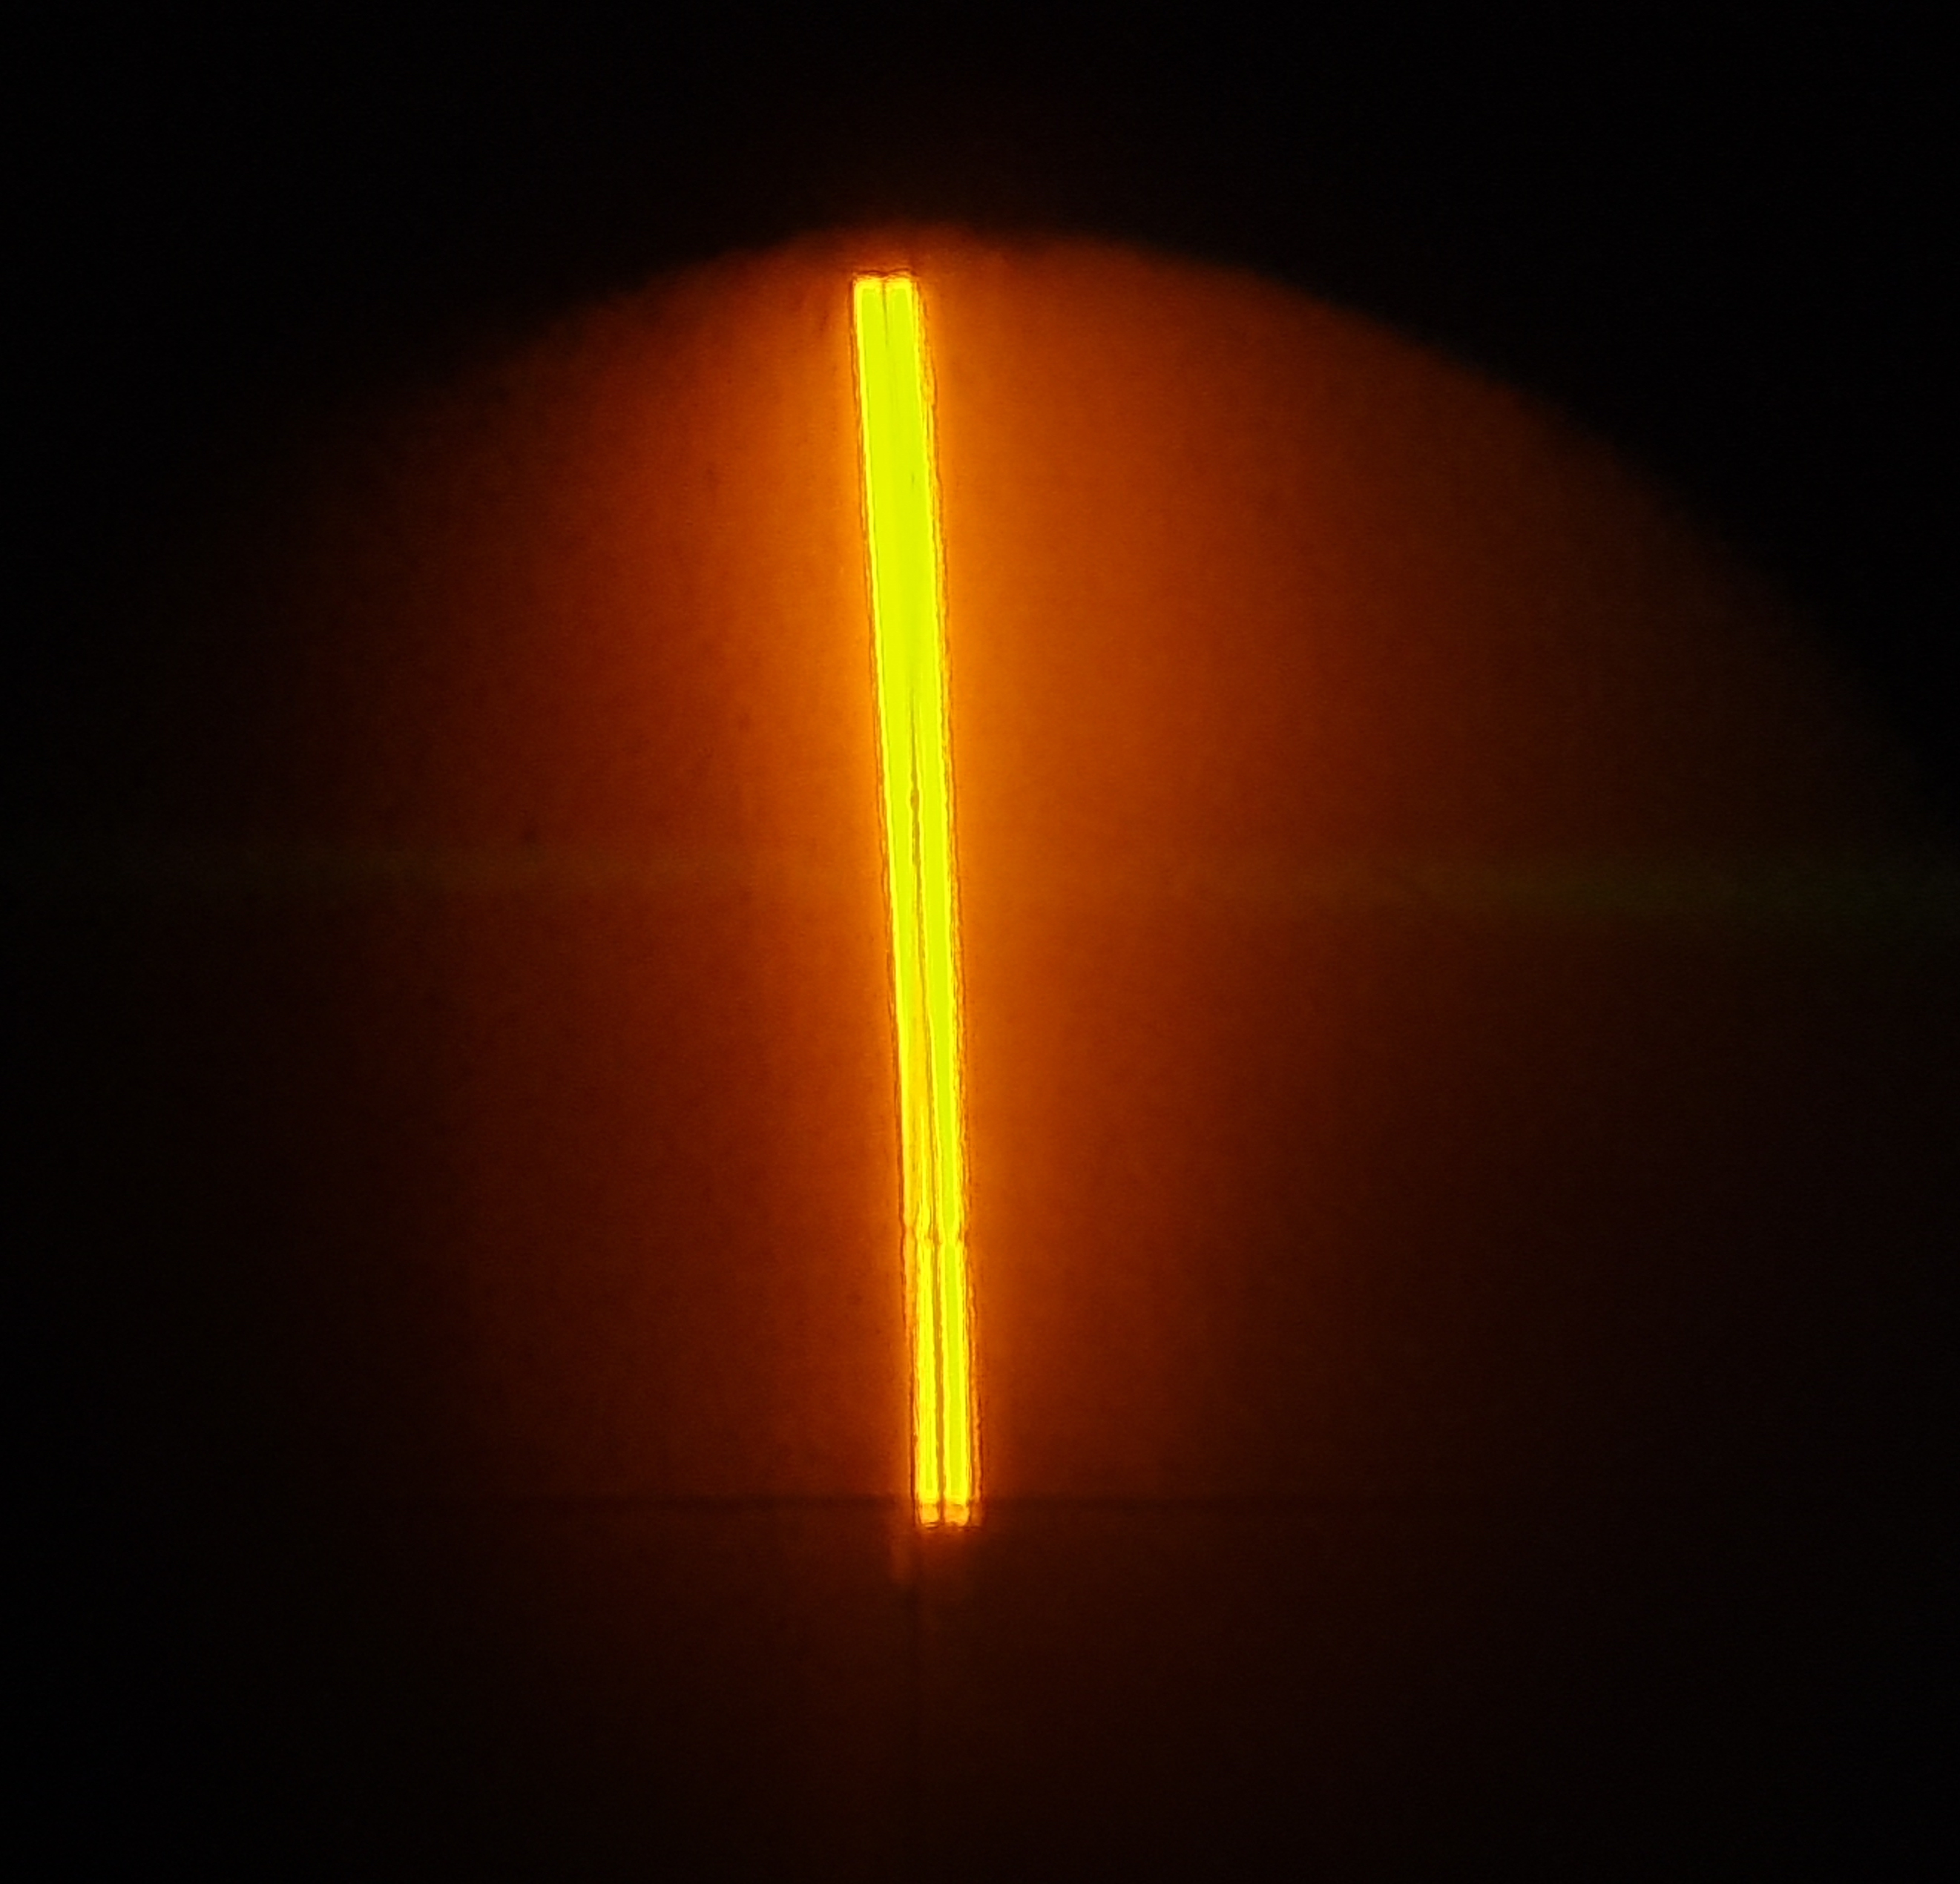
\includegraphics[width=8.3cm]{3} 
	\caption{First order Sodium Doublet visible through eye piece}
	\label{1}
\end{figure}

We could observe the sodium doublet with a very small gap between them. Only first order and second order was prominently visible through the spectrometer, Hence readings for greater than second order could not be taken.   

To calculate the $\lambda$ the equation (1)  changes to 
\begin{equation}
	\lambda_1=\frac{sin \theta_1}{N} \text{ and } 	\lambda_2=\frac{sin \theta_2}{N}
\end{equation}

From the analysis, for the first order we obtained $\lambda$'s as 596.057 nm and 595.840 nm with a difference 0.217 nm; for the second order $\lambda$'s as 618.508 nm and 617.766 nm with a difference 0.742 nm. The average of the difference of wavelength $\approx$ 0.480 nm. 

To calculate angular dispersive power equation (2) becomes

\begin{equation}	\frac{d\theta}{d\lambda}=\frac{mN}{cos\theta}
\end{equation}
where $\theta$ is average $\theta$ for the doublet.

For first order, average $\theta$ is $20.951^{\circ} $ (0.3656 rad)
\begin{equation}	\frac{d\theta}{d\lambda}=\frac{600}{cos (0.3656)}=642.476 ~rad / mm
\end{equation}

For second order, average $\theta$ is $47.882^{\circ} $ (0.8357 rad)
\begin{equation}	\frac{d\theta}{d\lambda}=\frac{2\times600}{cos (0.8357)}= 1789.286~rad / mm
\end{equation}
	
Propagation of error can be calculate as follows-
\begin{equation}
	\delta \lambda=\frac{cos\theta. \delta \theta}{m.N}
\end{equation}

where $\delta \theta$ is the least count for the spectrometer (10'') and N=1200 lines/mm.

From equation (7), we get for first order $\delta \lambda_1$=4.326 nm and $\delta \lambda_2$=4.327 nm and for second order $\delta \lambda_1$=1.552 nm and $\delta \lambda_2$=1.554 nm.

For difference in wavelengths, error can be calculated as 

\begin{equation}
	\delta(\Delta \lambda^1)=\sqrt{(\delta \lambda_1)^2+\delta( \lambda_2)^2}
\end{equation}
 For the first order,
 \begin{equation}
	\delta(\Delta \lambda^1)=\sqrt{(4.326)^2+\delta(4.327)^2}=6.118~nm
 \end{equation}
 For the second order,
 \begin{equation}
	\delta(\Delta \lambda^2)=\sqrt{(1.552)^2+\delta(1.554)^2}=2.196~nm
\end{equation}

For average $\Delta \lambda^{avg}$,
\begin{equation}
		\delta(\Delta \lambda^{avg})=\sqrt{(6.118)^2+\delta(2.196)^2}=6.500~nm
\end{equation}

\section{Conclusion}
The wavelength of sodium doublet by using the diffraction grating was found to be $\lambda_1=(596.057\pm4.326) nm $ and $\lambda_2=(595.840\pm4.327) nm $ for the first order diffraction pattern and  $\lambda_1=(618.508\pm1.552) nm $ and $\lambda_2=(617.766\pm1.554) nm $ for the second order diffraction pattern. The difference in wavelength was found to be  $\Delta \lambda^1=(0.217\pm6.118)$ nm for the first order and $\Delta \lambda^2=(0.742\pm2.196)$ nm for the second order. The average of differences of $\lambda_1$ and $\lambda_2$ was found to be $\lambda^{avg}$=$(0.480\pm6.5)$ nm. The angular dispersion was also calculated for the first order and second whose values are $642.476 ~rad / mm$ and $1789.286 ~rad / mm$, respectively. 

The values of wavelength from first order is close to the literature value of the sodium but for the second order, we started the experiment with the initial light of the sodium lamp resulting in higher wavelength than normal value. Moreover, the difference of wavelengths was not measured directly, the error sky-rockets the value. Through this experiment we could resolve up to two orders of diffraction pattern from the grating of 600 lines/mm. The instrumental errors accounts for most of the errors in the calculation as there is some involuntary movement of the slits of the apparatus while measuring the pattern from the fixed position. The main scale and vernier scale should are not tight enough and stable to take the measurements adding it to the error. Some amount of human error may also pop up while taking the fine readings of the spectrometer as it easy to misread the scale. The coinciding the edge of the pattern  and cross-wire of the telescope is also a guess as it is hard to align through eyes. It should be noted that the apparatus should be locked while taking readings and fine adjustment should be used and moved in only one direction to avoid the backlash error.  This experiment was successful in resolving the sodium light into two lines and gave a rough estimate about the difference of doublet.

\section{References}
\begin{enumerate}
\item{\url{https://www.niser.ac.in/sps/sites/default/files/basic_page/Sodium%20D%20line%20splitting.pdf}}
\item{\url{https://www.chem.uci.edu/~unicorn/249/Handouts/RWFSodium.pdf}}
\end{enumerate}
\end{document}